L'objectif de cette semaine est de pouvoir générer un jeu de données pour la validation croisée sous weka.

\subsection{Classer les données}

Avant de poursuivre, la base de donnée à été modifiée afin des données classée. Ceci permet de mieux se retrouver entre séquences d'acides aminées, nucléotidiques, fichier genbank, les enzymes (cox1,cox2...) ...

~\\
Chaque dossier comporte en plus des dossiers des sous taxons:

\begin{itemize}
 \item[.]Un dossier \textit{frequencies} où sera rangées les fréquences de kmers
  \item[.]un dossier \textit{data} correspondant aux données génétiques et étant constitué
  \begin{itemize}
 \item Un dossier \textit{fasta} où sera rangées les séquences, constitué de deux sous dossiers 
  \begin{itemize}
 \item[*]\textit{aminoAcids} contenant les séquences d'acides aminés, chaque cox, cytb,...sont également rangé dans un dossier de même nom. 
 
  \item[*]\textit{nucletotides} contenant les séquences nucléotidiques, de même ici chaque cox, cytb,...sont également rangé dans un dossier de même nom. Ce dossier contient en plus un dossier \textit{genomes} contenant tous le génome complet (voir figure \ref{dossierCox}).
  
\end{itemize}
  \item un dossier \textit{genbank} contenant les fichiers genbank associés au taxon courant
  
\end{itemize}
\end{itemize}
~\\

\begin{figure}[H]
\begin{center}
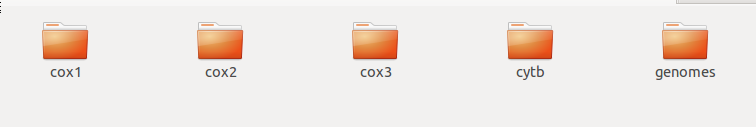
\includegraphics[scale=0.5]{./../img/dossier.png}
\caption{\label{dossierCox} Dossiers lorsqu'on se trouve dans le dossier data/fasta/nucleotides d'un taxon.}
\end{center}
\end{figure}
~\\

Cette façon de classer les données permet à l'utilisateur de pouvoir spécifier sur quelles séquences il souhaites travailler en indiquant les mots clés \textit{cox1},\textit{cox2},...ou \textit{genomes}.
